% Chapter Template

\chapter{Introducción específica} % Main chapter title

\label{Chapter2} % Change X to a consecutive number; for referencing this chapter elsewhere, use \ref{ChapterX}

%----------------------------------------------------------------------------------------
%	SECTION 1
%----------------------------------------------------------------------------------------
En el presente capítulo se introducen los módulos principales del equipo dip coater fabricado.   

\section{Estudio preliminar}

Para entender la relación entre la velocidad de extracción y el espesor de material depositado se tuvo en consideración la siguiente publicación \textit{(Preparation of Sol-Gel Films by Dip-Coating)} \cite{paper_galo}, que describe la técnica dip coating como un proceso dinámico, complejo, difícil de modelar, debido a los gradientes de concentración y viscosidad generados por evaporación de la solución. 


La publicación se basa entonces en un estudio semi-experimental sobre varias soluciones químicas para predecir el espesor final de la película. Tiene en cuenta dos modelos matemáticos, un modelo de capilaridad asociado a extracciones en velocidades bajas y otro modelo de evaporación asociado a velocidades altas respecto al rango de estudio. 

Se observa en la figura \ref{fig:paper_galo} la variación de los espesores fabricados respecto a velocidades utilizadas, también se puede observar la relación entre los diferentes modelos aplicados. 

\begin{figure}[!h]
\centering 
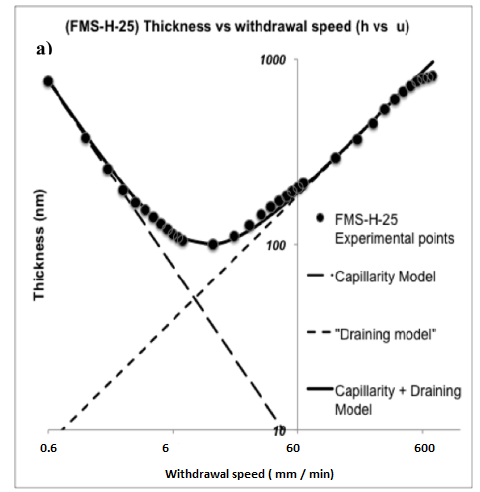
\includegraphics[width=0.52\textwidth]{./Figures/paper_galo.png}
\caption{Espesor vs velocidad \protect\footnotemark.}
\label{fig:paper_galo}
\end{figure}

\footnotetext{Imagen tomada de \cite{paper_galo}.}


Los resultados del experimento concluyen que existe linealidad  en la relación de espesor respecto la velocidad de extracción entre \SI{60}{\milli\meter\per\minute} y \SI{600}{\milli\meter\per\minute} . También demuestra que en dicho rango de velocidades el fenómeno se explica por el modelo de evaporación.

Se desprende de este análisis la importancia de los siguientes requerimientos funcionales definidos por el cliente: 

\begin{itemize}
\item El sistema debe contar con un rango de velocidades de desplazamiento de muestra entre [1- 1000 \si{\milli\meter\per\minute}]. 
\item El sistema debe contar con un rango de aceleraciones de desplazamiento de muestra entre [1000 - 15000 \si{\meter\per\square\minute}].
		
\end{itemize}
	
Cabe destacar que todos los experimentos en la publicación fueron realizados a velocidad constante. De las reuniones con el cliente y del interés de trabajar en la frontera de la ciencia surgió la necesitad de poder darle al usuario la posibilidad de realizar experimentos a velocidad y aceleración controlada. Esto último es una cualidad que diferencia a este equipo respecto de todos los equipos comerciales analizados en la sección \ref{sec:mercado}.

 
%Sin embargo, es una técnica muy difundida porque es simple y proporciona una excelente reproducibilidad. 
%El problema con este modelo es que la mayoría de las soluciones utilizadas son fluidos no-newtonianos, %es decir en donde el solvente de la solución se va evaparonado en simultáneo con la extracción de la %muestra induciendo una modificación en la densidad, tensión superficial y viscosidad del fluido. 
%Existen modelos matemáticos basados en la mecánica newtoniana que no tienen en cuenta la evaporación de %las soluciones y requieren varias suposiciones y simplificaciones. En estos modelos llegar a la %predicción del espesor depende de la densidad, la tensión superficial y la viscosidad del fluido. 
%La importancia de estos resultados es que el rango de velocidades quedá incluido dentro de los %requerimientos de nuestro equipo. 


\section{Circuitos integrados Trinamic}

%De los siguientes requerimientos funcionales acordados con el cliente:
De reuniones con el cliente en donde se remarca la importancia de trabajar con un control preciso de motor y en base a experiencias de uso de equipos con tecnologías similares surge el interés de trabajar con un fabricante de driver específico. Se definen entonces los siguientes requerimientos:
			
\begin{itemize}
\item El equipo deberá contar con un motor paso a paso Nema 17 \citep{web_nema17}  para realizar los movimientos.
\item Se utilizará un driver de motor de la marca TRINAMIC.
\end{itemize}

\textit{Trinamic Motion Control} \citep{3_web_trinamic} se especializa en la fabricación de CI (Circuitos Integrados) para el control de diferentes tipos de motores, su lema se basa en convertir señales digitales en movimientos controlados. Tiene una experiencia de veinte años en la industria del control de motores, lo que garantiza en cierta medida la calidad de sus productos, actualmente fue adquirida por la compañía Analog Devices \citep{web_analogdevices}.

Cabe destacar que los integrados fabricados por la empresa Trinamic se utilizan en diversas aplicaciones en donde la precisión es importante, como por ejemplo impresión 3D, automatización industrial, robótica y equipos de laboratorio médico entre otras.
Cuenta con una amplia gama de productos que se diferencian principalmente según el tipo de motor que se quiera accionar. Luego de estudiar las diferentes alternativas ofrecidas se eligió trabajar con el driver TMC5130 \citep{3_web_trinamic_producto}.
  
Todos los CI requieren una configuración inicial de parámetros, que dependen del tipo de  motor y de la carga asociada al mismo. Es por eso que la empresa ofrece el software TMCL-IDE  y diferentes placas de desarrollo para ayudar a realizar una correcta configuración de parámetros. La placa de desarrollo para este integrado es la \textit{TMC5130-Eval Evaluation Board} \citep{3_web_trinamic_placa}.

El TMCL-IDE se ejecuta sobre una placa de desarrollo general compatible con diferentes kits de evaluación. En la figura \ref{fig:tmc5130_placa} se observa a izquierda la placa Startrampe  que se conecta entre la computadora y la placa de evaluación \textit{TMC5130-Eval} que se observa a derecha. Finalmente el motor paso a paso se conecta a la placa de evaluación.

\begin{figure}[htpb]
\centering 
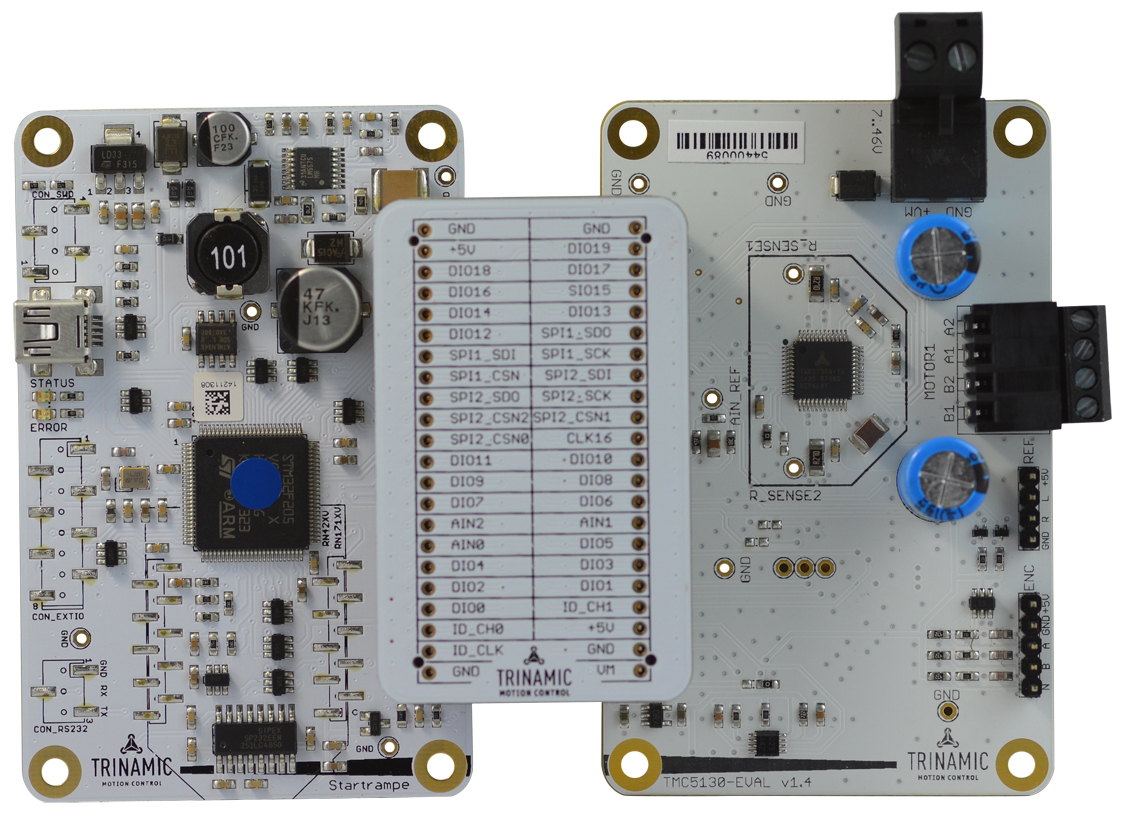
\includegraphics[width=0.9\textwidth]{./Figures/tmc5130_placa.jpg}
\caption{Placa de desarrollo Startrampe + placa de evaluación TMC5130 \protect\footnotemark.}
\label{fig:tmc5130_placa}
\end{figure}

\footnotetext{Imagen tomada de \cite{3_web_trinamic}.}


  
\subsection{Driver TMC5130}

El driver TMC5130 permite operar motores bipolares de dos fases comúnmente conocidos como motores paso a paso. El CI incorpora una etapa de potencia con tecnología \textit{MOSFET (Metal Oxide Semiconductor Field Effect Transistor)}  que permite manejar corrientes de hasta dos amperios por fase. En el caso de nuestro dip coater el peso de la carga es despreciable, por lo tanto la corriente es suficiente. Se realizarán en el capítulo \ref{Chapter4} los respectivos ensayos.

Podemos observar en la figura \ref{fig:tmc5130_diagrama} el diagrama en bloque del CI.

\begin{figure}[htpb]
\centering 
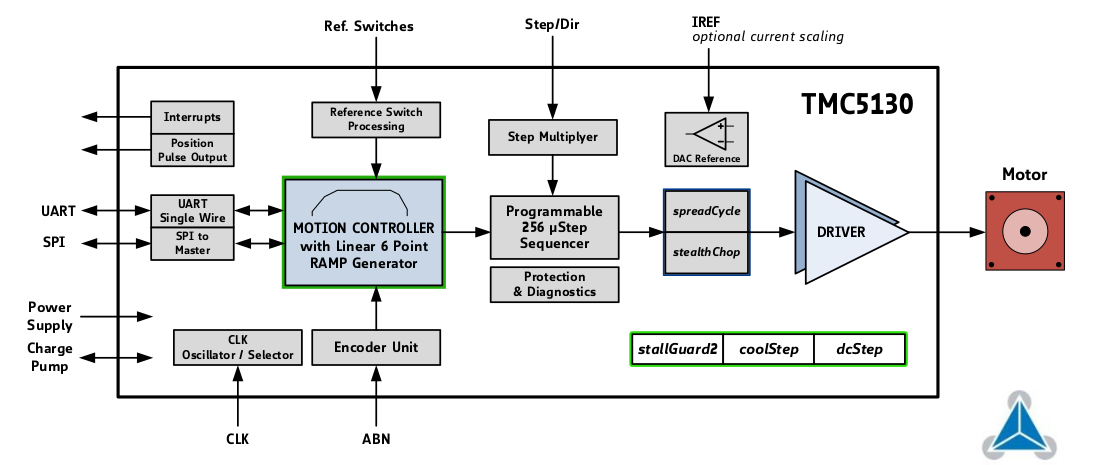
\includegraphics[width=1.1\textwidth]{./Figures/tmc5130_diagrama.png}
\caption{Diagrama en bloques TMC5130 \protect\footnotemark.}
\label{fig:tmc5130_diagrama}
\end{figure}

\footnotetext{Imagen tomada de \cite{3_web_trinamic}.}

La comunicación con el CI se puede establecer a través del protocolo \textit{ UART (Universal Asynchronous Receiver-Transmitter)} o \textit{SPI (Serial Peripheral Interface)}, en el caso de nuestro equipo utilizaremos la comunicación SPI.


Una característica importante a destacar es la posibilidad de programar la cantidad de pasos que da el motor. Los pasos están relacionados con las fases  y con la cantidad de dientes que tiene el rotor y estator del motor. Un paso es el movimiento mínimo que el motor puede hacer. Un motor paso a paso, como su nombre lo indica, realiza movimientos a través de pasos sucesivos. Por ejemplo es común contar con algún motor en donde la especificación dice que el paso es de (\ang{1.8}), esto significa que por cada vuelta de motor (\ang{360}) el motor realizará 200 pasos.

Una funcionalidad que incorpora este CI es incrementar la cantidad de pasos, el fabricante los denomina micropasos, el driver puede generar hasta un máximo de 256 micropasos por cada paso del motor. Siguiendo con el ejemplo recién presentado, para un motor de paso (\ang{1.8}) tendríamos en total 51200 micropasos como se observa en la ecuación \ref{eq:micro_pasos}.

\begin{equation}
	\label{eq:micro_pasos}
		(360/1.8) * 256 = 51200 \textup{ micropasos por revolución}
\end{equation}

En nuestro equipo el motor estará acoplado a un eje lineal para generar un movimiento. Por lo tanto cada micropaso del motor estará asociado a un desplazamiento lineal que se analizará en el capítulo \ref{Chapter3}.

Otra funcionalidad que se utilizará es \textit{Stallguard2}, una función de alta precisión que mide la fuerza contraelectromotriz generada en la bobinas del motor por cambios de carga en el eje. Como se observa en la figura \ref{fig:tmc5130_stallGuard2} el valor de stallguard se decrementa linealmente a medida que la carga en el eje del motor aumenta. En nuestro caso se utilizará esta funcionalidad para realizar un posicionamiento inicial que servirá de referencia para todos los desplazamientos posteriores. Cada vez que el equipo se enciende que ejecuta esta funcionalidad para buscar el respectivo cero de máquina.
     
\begin{figure}[htpb]
\centering 
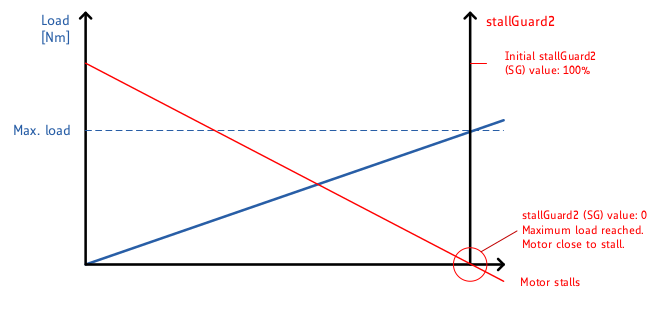
\includegraphics[width=0.9\textwidth]{./Figures/tmc5130_stallguard2.png}
\caption{Función stallGuard2.}
\label{fig:tmc5130_stallGuard2}
\end{figure}

También se utilizará \textit{coolStep}, una función que a través de mediciones de carga en el eje del motor adapta automáticamente la corriente suministrada hacia las bobinas, aumentando la eficiencia como puede observarse en la figura \ref{fig:tmc5130_coolStep}, cuyo efecto reduce la energía según hojas de datos \citep{3_web_trinamic_producto} hasta un \SI{75}{\percent}. Incluso en aplicaciones en donde la carga es constante como es el caso de nuestro equipo.

\begin{figure}[htpb]
\centering 
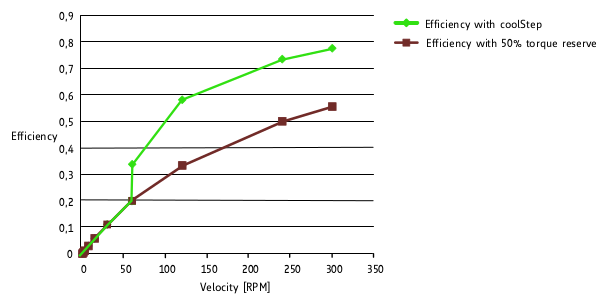
\includegraphics[width=0.9\textwidth]{./Figures/tmc5130_coolstep.png}
\caption{Función coolStep.}
\label{fig:tmc5130_coolStep}
\end{figure}

Por último se utilizará la función \textit{dcStep}, que es un modo de conmutación automática que ajusta la velocidad del motor en caso de existir cierta sobrecarga sobre el eje, es decir que si no puede mover la carga acoplada al eje con la velocidad establecida se ajusta a una velocidad menor para poder seguir en movimiento y no detenerse por completo. 


%el capítulo \ref{Chapter3} se darán detalles de las configuraciones finales del equipo.
El driver TMC5130 cuenta con 50 registros que se utilizan para configurar las funcionalidades del CI y controlar el motor conectado. El acceso a los registros se realizará a través del protocolo SPI. En el capítulo \ref{Chapter3} de darán mas detalles de los registros configurados con la ayuda del software TMCL-IDE.  


\section{Interfaz de usuario}

Respecto a la interfaz usuario-máquina surgió en reuniones con el cliente la necesidad de contar con una interfaz moderna, que permita a un usuario dentro de un laboratorio configurar el equipo a pie de máquina. 

Dando lugar al siguiente requerimiento:
\begin{itemize}
\item La configuración de la máquina debe poder realizarse a través de una pantalla táctil.	
\end{itemize} 

Se decidió trabajar con pantallas del tipo \textit{HMI (Human Machine Interface)}, este tipo de pantallas incorpora una unidad de procesamiento que se encarga exclusivamente del procesamiento gráfico. Cuentan con un software de diseño para la creación de la interfaz gráfica, que a través de un protocolo de comunicación definido por cada fabricante interactúa con el sistema de control, permitiendo finalmente controlar y configurar el equipo. En nuestro caso la pantalla se comunica con un microcontrolador, pero  podría  comunicarse con algún otro sistema de control como por ejemplo un  \textit{PLC (Programmable Logic Controller)}, 
 

Luego de una investigación de mercado se eligió a la empresa STONE \citep{web_stone}. El fabricante ofrece un catálogo amplio de equipos y en nuestro caso por las dimensiones finales del equipo se optó por pantallas de 4.3 pulgadas. Se detalla en la tabla \ref{tab:tabla_stone} las características técnicas de dos pantallas de 4.3 pulgadas del fabricante.

\begin{table}[!ht]
	\centering
	\caption[Comparación Stone]{Comparación pantallas táctiles Stone 4.3.}
	\begin{tabular}{l c c }    
		\toprule
		\textbf{}     & \textbf{STWI043WT} & \textbf{STVI043WT} \\
		\midrule
		CPU 			& 	Cortex A8         		& 	CortexM4 			 	\\		
		Refresh Rate    & 	1G Hz         			& 	200 MHz 				\\
		Image format  	& 	png,bmp,jpg,svg,gif     & 	bmp,jpg 				\\
		Resolution		& 	480×272 pixel	        & 	480×272 pixel 			\\
		Flash  			& 	256MB         			& 	128MB 					\\
		Color  			& 	262 K	          		& 	65 K 					\\
		PCB 			& 	2.0mm black, ROHS       & 	1.6mm green 			\\
		Touch Type		& 	Resistive    			& 	Resistive				\\
		Interface 		& 	RS232/RS422/RS485/TTL   & 	RS232/RS485/TTL			\\
		\bottomrule
		\hline
	\end{tabular}
	\label{tab:tabla_stone}
\end{table}


El modelo elegido fue el STWI043WT, que pertenece a la nueva línea productos, tiene mayor capacidad de procesamiento, cuenta con un software nuevo de configuración con mayores funcionalidades respecto al utilizado por el otro modelo y la diferencia de precios no supera el \SI{15}{\percent}.  

La comunicación de la pantalla STWI043WT con el microcontrolador se realizará a través del protocolo UART.


%El modelo elegido como se observa en la figura \ref{fig:stone}
%\begin{figure}[htpb]
%\centering 
%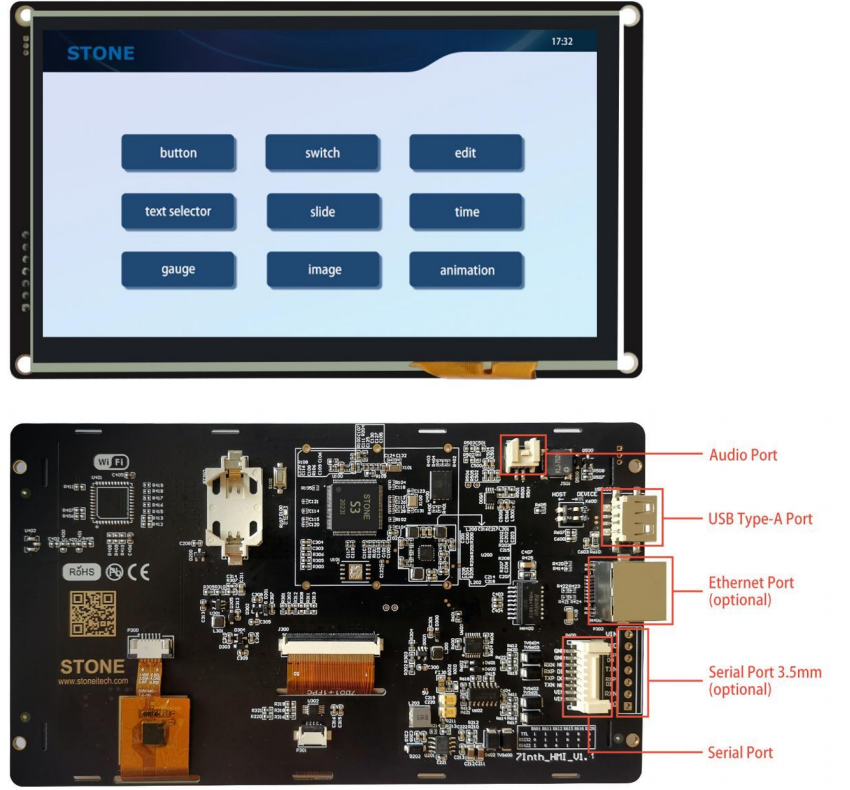
\includegraphics[width=0.5\textwidth]{./Figures/stone.png}
%\caption{Display táctil Stone.}
%\label{fig:stone}
%\end{figure}

\section{Estructura mecánica}
\label{sec:estructura_mecanica}

Se presentan a continuación los siguientes requerimientos asociados a las partes mecánicas del equipo: 

\begin{itemize}
\item La estructura principal del equipo debe ser fabricada con perfil de aluminio anodizado natural.
\item El recorrido mecánico de desplazamiento de muestra debe ser como mínimo de [3500 mm].
\item Las piezas especiales del equipo deben ser mecanizadas en aluminio.

\end{itemize}

Se decidió trabajar con el proveedor Perfiles de Aluminio .NET \citep{web_perfiles_net}, que cuenta con diferentes modelos y dimensiones de perfiles necesarios para la fabricación de la estructura.

El equipo también contará con una guía lineal acoplada al perfil principal. Para la elección de la guía se tuvieron en cuenta las siguientes consideraciones:

\begin{enumerate}
\item El ambiente cambia  según las soluciones químicas utilizadas. Es posible entonces que se trabaje con soluciones corrosivas que afecten la estructura.  
\item El uso de lubricantes en las guías podría afectar la calidad del experimento.
\item Se deben evitar vibraciones en la estructura para no dañar la calidad del \textit{film}.

\end{enumerate}

Se decidió entonces trabajar con la empresa IGUS \citep{web_igus}, que se especializa en la fabricación de polímeros. La empresa ofrece guías lineales que se deslizan en lugar de rodar, es decir no tienen rodamientos. Los polímeros están combinados con materiales anticorrosivos y no requieren la aplicación de lubricante, es decir que conforman un entorno de trabajo limpio y libre de mantenimiento periódico. Se observa en la figura \ref{fig:equipo_mecánico} cuatro tipos de guías en donde se puede apreciar el polímero auto-lubricado que se ubica entre el eje y el carro.

\begin{figure}[ht]
\centering 
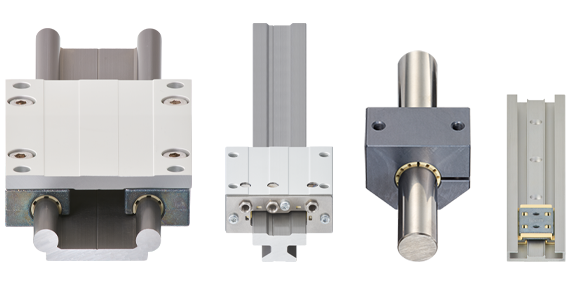
\includegraphics[width=0.7\textwidth]{./Figures/guias.png}
\caption{Guía Lineal IGUS.}
\label{fig:equipo_mecánico}
\end{figure}

Para el diseño y fabricación de piezas mecanizadas en aluminio se trabajó con el software BOBCAD \citep{web_bobcad} \textit{CAD/CAM (Computer-Aided Design /Computer-Aided Manufacturing )}. Un software  utilizado en la industria manufacturera compuesto por dos módulos fundamentales que abarcan los aspectos de diseño y luego de respectiva fabricación.  

Con la parte CAD diseñamos un primer modelo 3D de pieza y antes de comenzar con el módulo CAM, realizamos  una impresión 3D con filamento PLA para probar las dimensiones y factibilidad de la pieza.
Una vez que el modelo queda aprobado comenzamos con el módulo CAM, este módulo se encarga de convertir el modelo 3D en lenguaje de máquina que el equipo puede interpretar.Se observa en la imagen \ref{fig:fagor} la fresadora \textit{ CNC (computer numerical control)} de la marca FAGOR \citep{web_fagor} disponible en el taller mecánico. El control de la fresadora interpreta el código G-CODE también conocido como RS-274 \citep{web_gcode} y lo convierte en los respectivos movimientos de motores.


\begin{figure}[ht]
\centering 
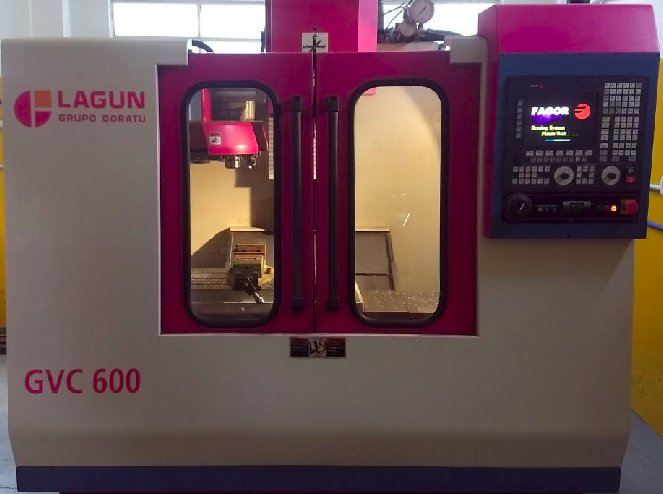
\includegraphics[width=0.7\textwidth]{./Figures/fagor.png}
\caption{Fresadora Fagor GVC 600.}
\label{fig:fagor}
\end{figure}
 

\section{Equipo electrónico propuesto}


Se presentan a continuación los siguientes requerimientos:
\begin{itemize}

\item El sistema debe permitir que el usuario pueda configurar en un programa variables de desplazamiento y tiempos de espera.
\item Un programa previamente configurado debe poder ejecutarse o guardarse en memoria interna.
\item El usuario debe poder guardar al menos 10 programas en la memoria no volátil del sistema.
\item Se deberá utilizar un control de versionado de cambios durante el desarrollo del firmware.
\item El desarrollo del firmware debe realizarse con capas de abstracción de software de tal manera que permita en un futuro cambiar de microcontrolador sin mayor esfuerzo.
\item El desarrollo de realizará sobre un módulo microcontrolador ESP32.
\item Deberá registrar variables de presión y temperatura [opcional].
\end{itemize}

De reuniones con el cliente y de la necesidad de trabajar con un equipo que permita a futuro contar con una comunicación Wi-Fi, surgió el requerimiento de trabajar con el módulo ESP32 \citep{web_esp}.
 
El ESP32 es un módulo del tipo \textit{SoC (system on a chip)} que integra mayores prestaciones a demás de su de unidad de procesamiento. Para almacenar los programas generados por el usuario se utilizará la memoria flash incorporada en el módulo.  

Teniendo en cuenta los requerimientos analizados en las secciones previas y los requerimientos analizados en esta sección se propone como puede observarse en la figura \ref{fig:equipo_propuesto} el siguiente esquema de equipo dip coater.  


\begin{figure}[ht]
\centering 
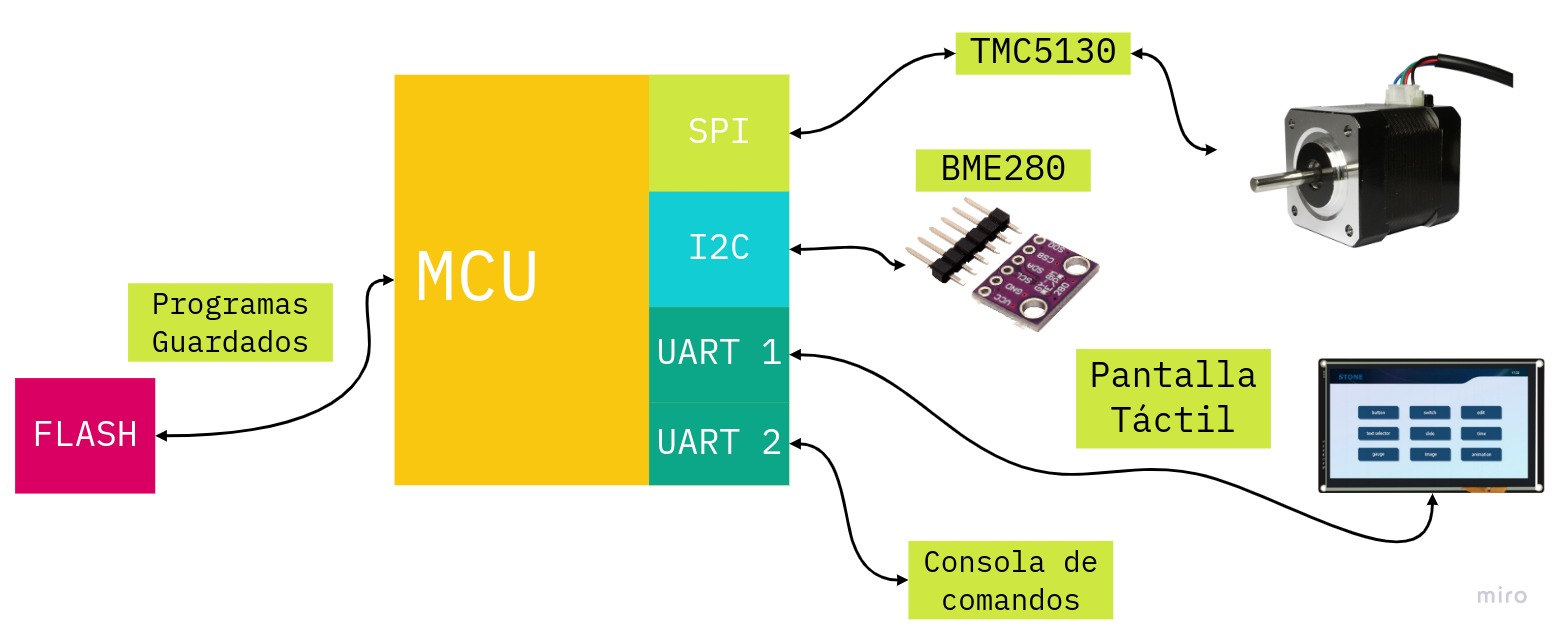
\includegraphics[width=0.9\textwidth]{./Figures/cap2_esquema_propuesto.jpg}
\caption{Esquema propuesto.}
\label{fig:equipo_propuesto}
\end{figure}

\begin{enumerate}
\item Módulo ESP32-WROOM. 
\item Consola de comandos para establecer una comunicación entre el equipo y una computadora (Protocolo UART)
\item Driver TMC5130 (Protocolo SPI).
\item Pantalla táctil STONE STWI043WT (Protocolo UART). 
\item Almacenamiento de programas (FLASH Interna).

\end{enumerate}


